\documentclass[a4paper,article,14pt]{extarticle}

\usepackage{spbudiploma}
\usepackage{amsmath}
\usepackage{mathtools}
\usepackage[pdftex]{graphicx}
\graphicspath{{../pictures/}}
\usepackage{listings}
\usepackage{xcolor}


\usepackage{enumitem}
\definecolor{codegreen}{rgb}{0,0.6,0}
\definecolor{codegray}{rgb}{0.5,0.5,0.5}
\definecolor{codepurple}{rgb}{0.58,0,0.82}
\definecolor{backcolour}{rgb}{0.95,0.95,0.92}

\lstdefinestyle{mystyle}{
	backgroundcolor=\color{backcolour},   
	commentstyle=\color{codegreen},
	keywordstyle=\color{codegreen},
	numberstyle=\tiny\color{codegray},
	stringstyle=\color{codepurple},
	basicstyle=\ttfamily\footnotesize,
	breakatwhitespace=false,         
	breaklines=true,                 
	captionpos=b,                    
	keepspaces=false,                 
	numbers=left,                    
	numbersep=5pt,                  
	showspaces=false,                
	showstringspaces=false,
	showtabs=false,                  
	tabsize=2
}

\lstset{style=mystyle}

\begin{document}
	\begin{titlepage}
		\begin{center}
			FEDERAL STATE AUTONOMOUS EDUCATIONAL INSTITUTION
			
			OF HIGHER EDUCATION
			
			ITMO UNIVERSITY
			\vspace{3cm}
			
			\large\textbf{Report}
			
			\large on the practical task No. 2
			
			\large \flqq Algorithms for unconstrained nonlinear optimization. \\ Direct methods\frqq
			\vspace{5cm}
			

			\begin{flushright}
				{Performed by:} \\
				Putnikov Semyon \\ 
				J4132c \\
			\end{flushright}
			
			
			\begin{flushright}
				{Accepted by:} \\
				Dr Petr Chunaev \\ 
			\end{flushright}
			\vfill
			
			{St. Petersburg}
			\par{\number\year}
		\end{center}
	\end{titlepage}

	\newpage
	
	\section{Goal}
	The use of direct methods (one-dimensional methods of exhaustive search, dichotomy, golden section search; multidimensional methods of exhaustive search, Gauss, Nelder-Mead) in the tasks of unconstrained nonlinear.
	
	\section{Formulation of the problem}
	\begin{enumerate}[label=(\Roman*)]
		\item\label{I} 
		Use the one-dimensional methods of exhaustive search, dichotomy and golden section search to find an approximate (with precision $\varepsilon = 0.001$) solution $x: f(x)\rightarrow min$ for the following functions and domains:
		\begin{enumerate}[label=(\arabic*)]
		    \item $f(x) = x^3,\quad x \in [0,1]$
		    \item $f(x) = |x - 0.2 |,\quad x \in [0,1]$
		    \item $f(x) = x\sin{\frac{1}{x}},\quad x \in [0.01,1]$
		\end{enumerate}
		Calculate the number of $f$-calculations and the number of iterations performed in each method and analyze the results. Explain differences (if any) in the results obtained.
		\item\label{II} 
		Generate random numbers $\alpha \in (0,1)$ and $\beta \in (0,1)$. Furthermore, generate the noisy data $\{x_k,y_k\}$, where $k = 0, \dotso, 100$, according to the following rule:
		$$y_k = \alpha x_k + \beta + \delta_k, \quad x_k = \frac{k}{100}$$
		where $\delta_k\: N(0,1)$ are values of a random variable with standard normal distribution. Approximate the data by the following linear and rational functions:
		\begin{enumerate}[label=(\arabic*)]
		    \item $F(x,a,b) = ax + b$ \quad (linear approximant),
		    \item $F(x,a,b) = \frac{a}{1+bx}$ \quad (rational approximant),
		\end{enumerate}
		by means of least squares through the numerical minimization (with precision $\varepsilon = 0.001$) of the following function: $D(a,b) = \sum\limits_{k=0}^{100} (F(x_k,a,b)-y_k)^2$
		
		To solve the minimization problem, use the methods of exhaustive search, Gauss and Nelder-Mead. If necessary, set the initial approximations and other parameters of the methods. Visualize the data and the approximants obtained in a plot separately for each type of approximant. Analyze the results obtained (in terms of number of iterations, precision, number of function evaluations, etc.).
	\end{enumerate}
	
	\section{Brief theoretical part}
	\subsection{Exhaustive search}
	
	In computer science, brute-force search or exhaustive search, also known as generate and test, is a very general problem-solving technique and algorithmic paradigm that consists of systematically enumerating all possible candidates for the solution and checking whether each candidate satisfies the problem's statement. A brute-force algorithm to find the divisors of a natural number n would enumerate all integers from 1 to n, and check whether each of them divides n without remainder.
	
	\subsection{Dichotomy method}
	
	Dichotomy method is a root-finding method that applies to any continuous functions for which one knows two values with opposite signs. The method consists of repeatedly bisecting the interval defined by these values and then selecting the subinterval in which the function changes sign, and therefore must contain a root.
	
	\subsection{Golden-section search}
	
	The golden-section search is a technique for finding an extremum (minimum or maximum) of a function inside a specified interval. For a strictly unimodal function with an extremum inside the interval, it will find that extremum, while for an interval containing multiple extrema (possibly including the interval boundaries), it will converge to one of them. If the only extremum on the interval is on a boundary of the interval, it will converge to that boundary point. The method operates by successively narrowing the range of values on the specified interval, which makes it relatively slow, but very robust.
	
	\subsection{Gauss method}
	
	Given $m$ functions $r = (r_1, \dotso, r_m)$ of $n$ variables $\beta = (\beta_1, \dotso, \beta)$, with $n \leq m$, algorithm iteratively finds the value of the variables that minimizes the sum of squares.
	$$S(\beta) = \sum\limits_{i=1}^m(r^2_i(\beta)$$
	Starting with an initial guess $\beta^{(0)}$ for the minimum, the method proceeds by the iterations $$\beta^{(s+1)} = \beta^{(s)} - (J_r^T J_r)$$
	where, if $r$ and $\beta$ are column vectors, the entries of the Jacobian matrix are
	$$(J_r)_{ij}=\frac{\partial r_i(\beta^{(s)})}{\partial \beta_j}$$
    In data fitting, where the goal is to find the parameters $\beta$ such that a given model function $y = f(x, \beta)$ best fits some data points $(x_i, y_i)$, the functions $r_i$ are the residuals: $r_i(\beta) = y_i - f(x_i, \beta)$.

	\subsection{The Nelder–Mead method}
	
	The Nelder–Mead method is a commonly applied numerical method used to find the minimum or maximum of an objective function in a multidimensional space. The method uses the concept of a simplex, which is a special polytope of n + 1 vertices in n dimensions. Examples of simplices include a line segment on a line, a triangle on a plane, a tetrahedron in three-dimensional space and so forth. The method approximates a local optimum of a problem with $n$ variables when the objective function varies smoothly and is unimodal. Typical implementations minimize functions, and we maximize $f(x)$ by minimizing $-f(x)$. Nelder–Mead in n dimensions maintains a set of $n + 1$ test points arranged as a simplex. It then extrapolates the behavior of the objective function measured at each test point in order to find a new test point and to replace one of the old test points with the new one, and so the technique progresses. The simplest approach is to replace the worst point with a point reflected through the centroid of the remaining n points. If this point is better than the best current point, then we can try stretching exponentially out along this line. On the other hand, if this new point isn't much better than the previous value, then we are stepping across a valley, so we shrink the simplex towards a better point.
	
	\section{Results}
	%Present the results of solving the assigned problems, including graphs and tables, as well as a brief discussion of the results obtained (at most 4 pages)
	
	\subsection{Task I}
	\subsubsection{Exhaustive search}
	
	At Figures \ref{cubeEx} we can see plot for functions I.1 from task description. It took 1000 steps to find minimum of this function because it exists on every point of viewed segment, so we need to check every point.
	
	At Figures \ref{moduleEx} we can see plot for functions I.2 from task description. It took 1000 steps to find minimum of this function as it was at previous run. 
	
	At Figures \ref{sinEx} we can see plot for functions I.3 from task description. It took less steps when later - only 990, because we have shorter for this function.
	
	\subsubsection{Dichotomy method}
	At Figures \ref{cubeDich} we can see plot for functions I.1 from task description. It took 11 steps to find minimum of this function.
	
	At Figures \ref{moduleDich} we can see plot for functions I.2 from task description. It took 11 steps to find minimum of this function.
	
	At Figures \ref{sinDich} we can see plot for functions I.3 from task description. It took 11 steps to find minimum of this function.
	
	This method showed better results than exhaustive search as expected, because this method have stronger optimization logic. We can see black points on the plots. It is intermediate values of calculation. 
	
	\subsubsection{Golden section method}
	At Figures \ref{cubeGolden} we can see plot for functions I.1 from task description. It took 15 steps to find minimum of this function.
	
	At Figures \ref{moduleGolden} we can see plot for functions I.2 from task description. It took 15 steps to find minimum of this function.
	
	At Figures \ref{sinGolden} we can see plot for functions I.3 from task description. It took 15 steps to find minimum of this function.
	
	This method showed worse result than dichotomy method. It took more steps than previous method. But golden section method needs less calculations of objective function. It can be important in some cases.
	
	We can see black points on the plots. It is intermediate values of calculation. 
	
	\subsection{Task II}
	\subsubsection{Exhaustive search (multidimensional)}
	
	At Figures \ref{linearEx} and \ref{rationalEx} we can see plots of function $D(a,b)$ with aproximation linear and rational functions respectively. Red points mean minimum of function $D(a,b)$.
	
	At both cases it took 10201 steps to find a minimum value, because we need to check every value of a grid.
	
	\subsubsection{Gauss method}
	
	At Figures \ref{linearGauss} we can see plot for functions $D(a,b)$ with linear aproximation. It took 4 steps.
	
	At Figures \ref{rationalGauss} we can see plot for functions $D(a,b)$ with rational aproximation. It took 3 steps.
	
	Gauss method showed the best results of calculation.
	
	\subsubsection{Nelder-Mead method}
	
	At Figures \ref{linearNM} we can see plot for functions $D(a,b)$ with linear aproximation. It took 50 steps.
	
	At Figures \ref{rationalNM} we can see plot for functions $D(a,b)$ with rational aproximation. It took 52 steps.
	
	\section{Conclusions}
	To sum it up, we’ve measured the amount of iterations of well-known algorithm implementations with specified values, using data plots, representing function and points of steps.
	
	After comparison of the empirical and theoretical calculation complexities we can say, that optimization algorithms can save time and computers resources. 
	
	\newpage
	\section{Figures}
	
	\begin{figure}[h]
		\centering
		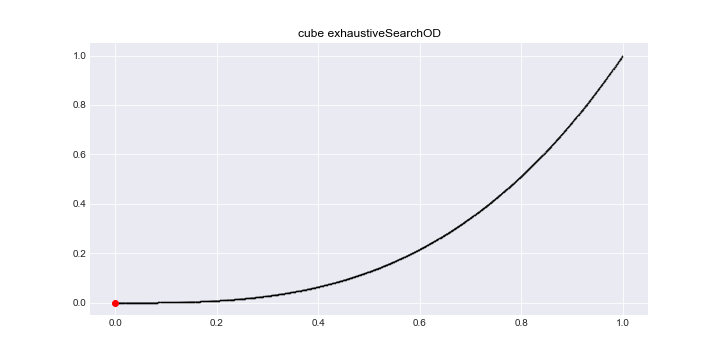
\includegraphics[scale=0.5]{cube_exhaustiveSearchOD.png}
		\caption{Function (I.1). Exhaustive search.}
		\label{cubeEx}
	\end{figure} 
	\begin{figure}[h]
		\centering
		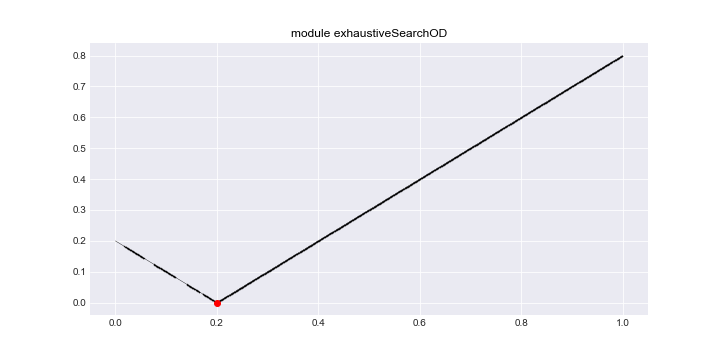
\includegraphics[scale=0.5]{module_exhaustiveSearchOD.png}
		\caption{Function (I.2). Exhaustive search.}
		\label{moduleEx}
	\end{figure} 
	\begin{figure}[h]
		\centering
		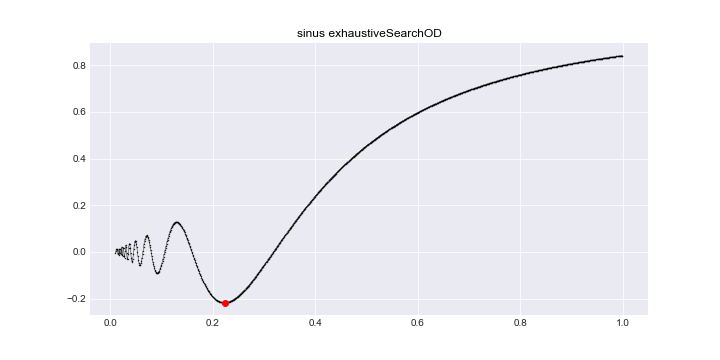
\includegraphics[scale=0.5]{sinus_exhaustiveSearchOD.png}
		\caption{Function (I.3). Exhaustive search.}
		\label{sinEx}
	\end{figure} 

	\begin{figure}[h]
		\centering
		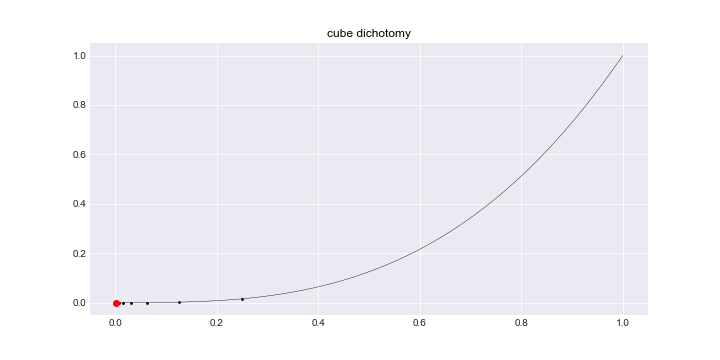
\includegraphics[scale=0.5]{cube_dichotomy.png}
		\caption{Function (I.1). Dichotomy method.}
		\label{cubeDich}
	\end{figure} 
	\begin{figure}[h]
		\centering
		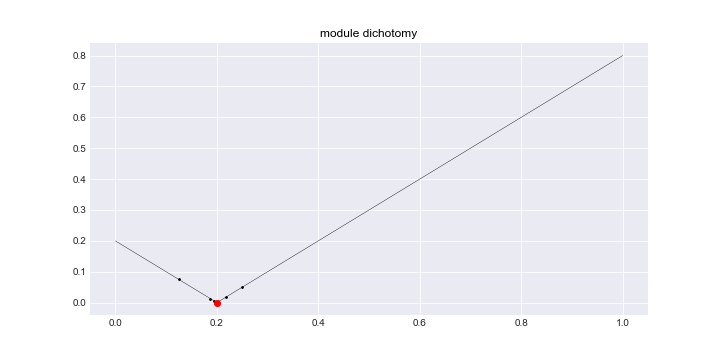
\includegraphics[scale=0.5]{module_dichotomy.png}
		\caption{Function (I.2). Dichotomy method.}
		\label{moduleDich}
	\end{figure} 
	\begin{figure}[h]
	\centering
	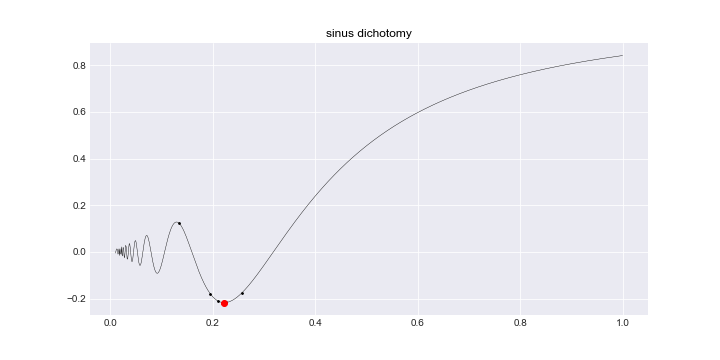
\includegraphics[scale=0.5]{sinus_dichotomy.png}
	\caption{Function (I.3). Dichotomy method.}
	\label{sinDich}
	\end{figure}

	\begin{figure}[h]
		\centering
		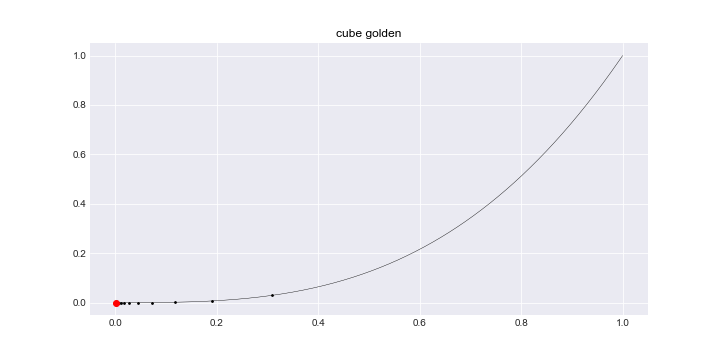
\includegraphics[scale=0.5]{cube_golden.png}
		\caption{Function (I.1). Golden section method.}
		\label{cubeGolden}
	\end{figure}
	\begin{figure}[h]
		\centering
		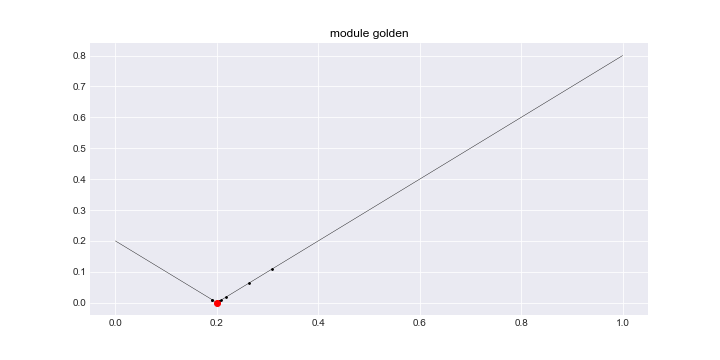
\includegraphics[scale=0.5]{module_golden.png}
		\caption{Function (I.2). Golden section method.}
		\label{moduleGolden}
	\end{figure}
	\begin{figure}[h]
		\centering
		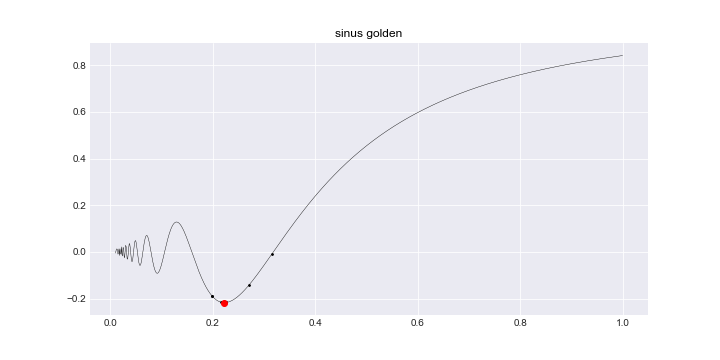
\includegraphics[scale=0.5]{sinus_golden.png}
		\caption{Function (I.3). Golden section method.}
		\label{sinGolden}
	\end{figure}
	
	\begin{figure}[h]
		\centering
		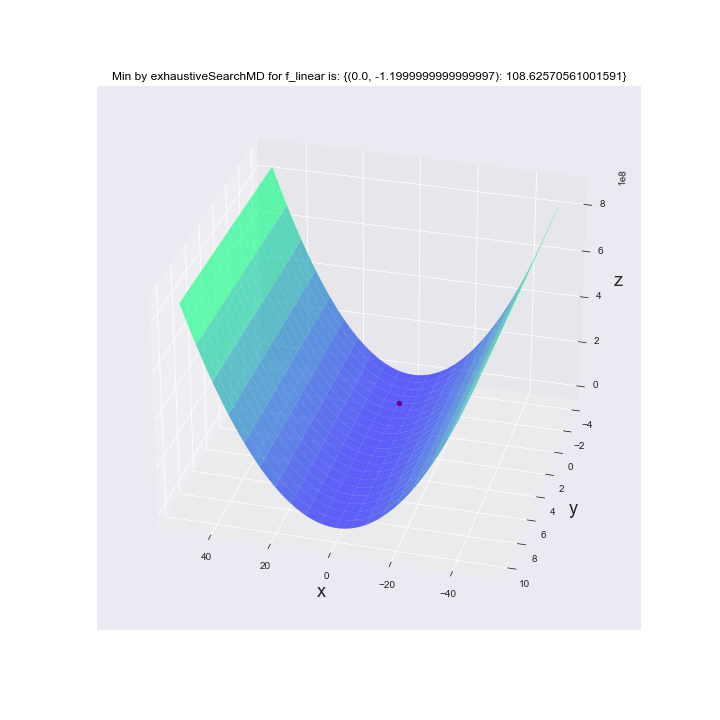
\includegraphics[scale=0.5]{f_linear_exhaustiveSearchMD.png}
		\caption{Linear approximant. Exhaustive search.}
		\label{linearEx}
	\end{figure} 
	\begin{figure}[h]
		\centering
		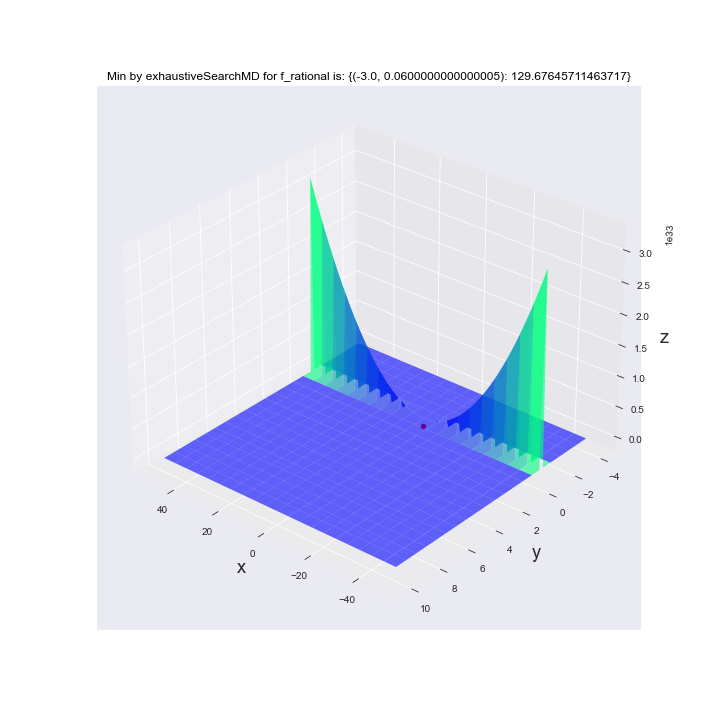
\includegraphics[scale=0.5]{f_rational_exhaustiveSearchMD.png}
		\caption{Rational approximant. Exhaustive search.}
		\label{rationalEx}
	\end{figure}

	\begin{figure}[h]
		\centering
		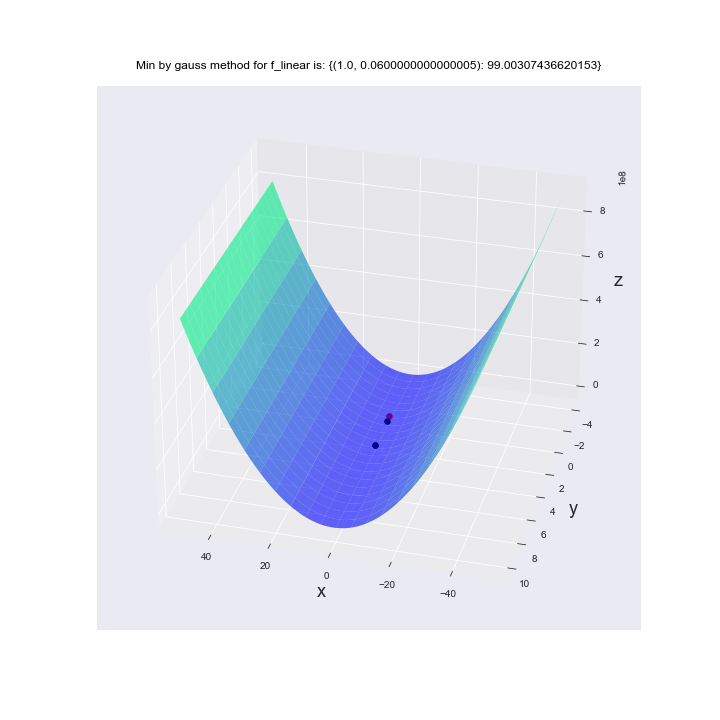
\includegraphics[scale=0.5]{f_linear_gauss.png}
		\caption{Linear approximant. Gauss method.}
		\label{linearGauss}
	\end{figure} 
	\begin{figure}[h]
	\centering
	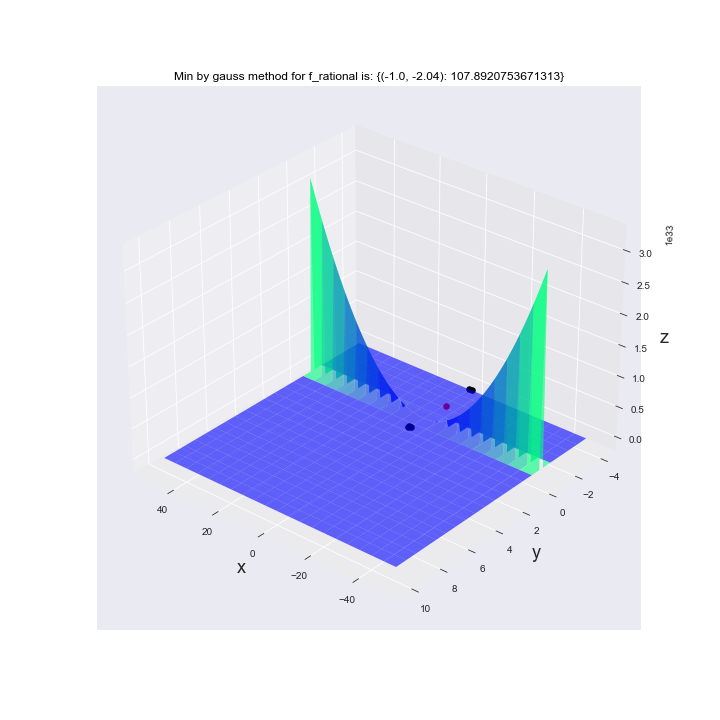
\includegraphics[scale=0.5]{f_rational_gauss.png}
	\caption{Rational approximant. Gauss method.}
	\label{rationalGauss}
	\end{figure} 

	\begin{figure}[h]
		\centering
		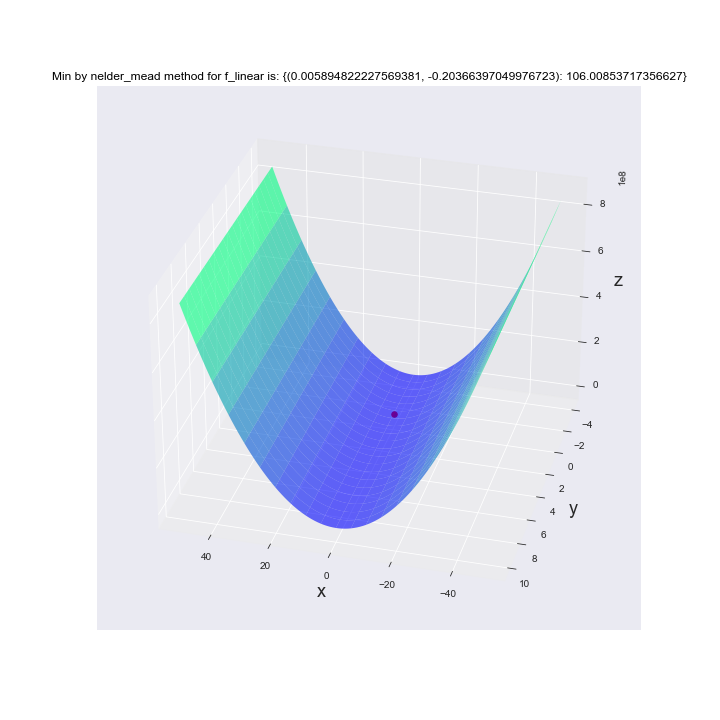
\includegraphics[scale=0.5]{f_linear_nelder_mead.png}
		\caption{Linear approximant. Nelder-Mead method.}
		\label{linearNM}
	\end{figure} 
	\begin{figure}[h]
		\centering
		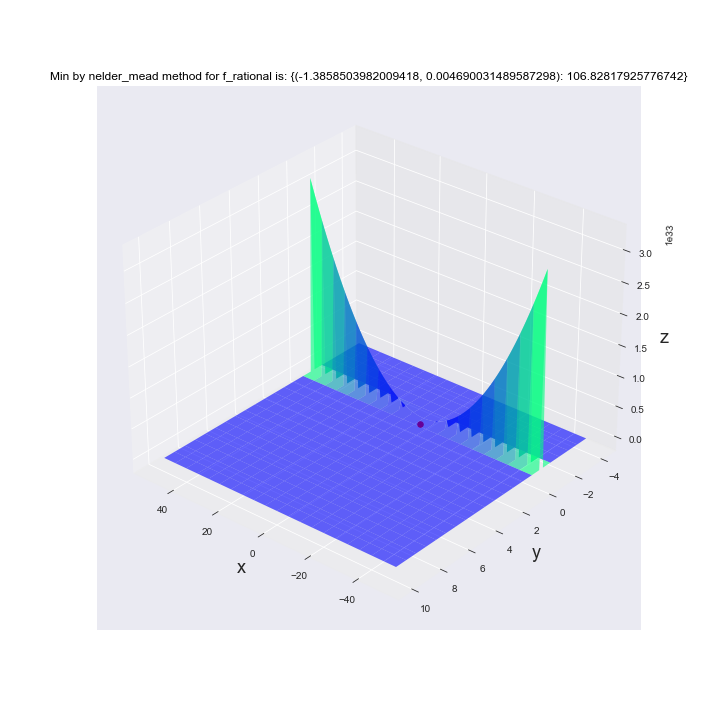
\includegraphics[scale=0.5]{f_rational_nelder_mead.png}
		\caption{Rational approximant. Nelder-Mead method.}
		\label{rationalNM}
	\end{figure} 
	
\end{document}